\section{Experiments}

\subsection{Experimental Setup}

The experiments are conducted on task graphs derived from real-world neural network models to ensure practical relevance. The task graphs are defined at tensor-level operations -- check the last statement. Each task graph represents a directed acyclic graph (DAG) where nodes correspond to computational tasks and edges represent data dependencies with. Since the graphs are generated by <\zmcomment{Placeholder for task graph generation description}>, we only obtain the topology. In order to test different partitioning methods on these task graphs, we have to assign costs associated with the nodes and edges. Extending Arato et al.~\cite{arato2005algorithmic}, we employ the following mechanism for task graph cost assignment.

\subsubsection{Cost Model}


\textbf{Software Execution Cost ($s_i$):} Represents the estimated execution time when task $i$ runs on a general-purpose processor. These costs are uniformly sampled in the range $[1, 100]$ to simulate varying computational complexity across different tasks.

\textbf{Hardware Execution Cost ($h_i$):} Represents the execution time when task $i$ is implemented as a dedicated hardware accelerator. The hardware cost is modeled as:
\begin{equation}
h_i = \max(0.1, \mathcal{N}(k \cdot  s_i, (l \cdot k \cdot s_i)^2))
\end{equation}
where $k > 0$ is the hardware scale factor and $l > 0$ is the hardware scale variance parameter. The scale factor $k$ determines the relative performance advantage of hardware implementation. During our implementation, we set $k < 1$ to indicate faster hardware execution time in general compared to its software execution counterpart. The variance parameter $l$ controls the variability in hardware costs relative to software costs, with smaller values maintaining a stronger correlation between $s_i$ and $h_i$.

\textbf{Hardware Area Cost ($a_i$):} Each hardware implementation incurs an area cost uniformly distributed in the range $[1, A_{max}]$, where $A_{max}$ represents the maximum area requirement for any single task. To impose area constraint, we define the area constraint ratio $\alpha$. Thus, any partitioning solution $\mathcal{P}$ should satisfy the following constraint $\sum_{i \in H_{\mathcal{P}}} a_i \leq \alpha \cdot \sum_i{a_i}$, where $H_{\mathcal{P}}$ is the set of tasks assigned to hardware as per partitioning $\mathcal{P}$.

\textbf{Communication Cost ($c_{i,j}$):} Represents the overhead incurred when data flows between tasks $i$ and $j$ assigned to different processing units. Communication costs are uniformly distributed in the range $[0, 2\mu \cdot s_{max}]$, where $s_{max} = \max_i(s_i)$ and $\mu$ is the communication scale factor. Higher values of $\mu$ increase the penalty for cross-platform communication, making partitioning decisions more critical for overall performance.

\subsubsection{Experimental Parameters}
The experimental evaluation employs the following parameter settings:
\begin{itemize}
    \item \textbf{Hardware Scale Factor ($k$):} Controls the relative hardware-software performance ratio
    \item \textbf{Hardware Scale Variance ($l$):} Determines cost correlation variability  
    \item \textbf{Communication Scale Factor ($\mu$):} Governs inter-partition communication overhead
    \item \textbf{Area Constraint ($\alpha$):} Fraction of total hardware area available for allocation
\end{itemize}

Configuration parameters are specified via YAML files, enabling systematic parameter sweeps and reproducible experimental conditions. Each experiment generates comprehensive logging and saves intermediate results including task graph instances, partition assignments, and performance metrics.

\subsubsection{Objective Functions}
The quality of the solution $\mathcal{P}$ is evaluated against six separate objective functions.

\textbf{ARATO:} The total cost, including execution costs and communication overhead:
\begin{equation}
C_{total} = \sum_{i \in S_{\mathcal{P}}} s_i + \sum_{i \in H_{\mathcal{P}}} h_i + \sum_{(i,j) \in E_{\mathcal{P}}} c_{i,j}
\end{equation}
where $S_{\mathcal{P}}, H_{\mathcal{P}}$ and $E_{\mathcal{P}}$ are software-assigned tasks, hardware-assigned tasks, and edges between tasks on different platforms induced by partitioning $\mathcal{P}$, respectively.

\zmcomment{This is a proxy cost of the actual cost as there are parallelism. Also serves as an upper bound. Similar cost was used in~\cite{arato2005algorithmic}}

\textbf{OPTM (One Possible Topological makespan):} While tasks assigned to software execute sequentially, hardware tasks can execute in parallel \zmcomment{cite a reference}, given the set of the precedence tasks have completed execution.

\zmcomment{This requires knowing the scheduling. How to write this part-- needs discussion.}

Here, we run the meta-heuristics to optimize one possible scheduling by choosing the lexicographically smallest possible topological ordering of the tasks at every point when there are multiple ready nodes, giving us one possible scheduling. Optimizing this objective function is more computationally extensive than the partition cost as it now requires one to run a $\mathcal{O}(n^2)$ heuristic \zmcomment{check with Rounak if the complexity is correct} to calculate the cost function during optimization.

Area constraint violations incur a penalty cost of $10^9$ to ensure feasible solutions, effectively treating the problem as a constrained optimization task. 

\textbf{CA (Communication-Aware):} \zmcomment{write about comm-aware heuristic}

\textbf{CPL (Critical Path List Scheduling):} \zmcomment{write about this heuristic}

\textbf{ED (Event-driven):} \zmcomment{write about event-driven heuristic}

\textbf{SPT (Shortest processing time):} \zmcomment{write about this heuristic}

Note that, during evaluations, all the solutions are evaluated using the OPTM strategy.

\zmcomment{this probably needs to be updated}

\subsection{Baseline Methods}

\begin{table}[htbp]
\centering
\caption{Parameter used for baseline methods. Numbers in bracket indicate changed values for OPTM objective function}
\label{tab:baseline_parameters}
\begin{tabular}{|p{0.15\textwidth}|p{0.45\textwidth}|p{0.2\textwidth}|}
\hline
\textbf{Algorithm} & \textbf{Parameter} & \textbf{Value} \\
\hline
\multirow{5}{*}{PSO} & Cognitive coefficient ($c_1$) & 0.575 \\
 & Social coefficient ($c_2$) & 0.1 \\
 & Inertia weight ($w$) & 1.05 \\
 & Population size & 500 \\
 & Iterations & 1000 (*10) \\
\hline
\multirow{7}{*}{DBPSO} & Cognitive coefficient ($c_1$) & 0.575 \\
 & Social coefficient ($c_2$) & 0.1 \\
 & Inertia weight ($w$) & 1.05 \\
 & Number of neighbors ($k$) & 4 \\
 & Minkowski p-norm ($p \in \{1,2\}$) & 2 \\
 & Population size & 500 \\
 & Iterations & 1000 (*10) \\
\hline
\multirow{3}{*}{CLPSO} & Comprehensive Learning Rate ($c$) & 1 \\
 & Population size & 500 \\
 & Iterations & 1000 (*200) \\
\hline
\multirow{3}{*}{CCPSO}
 & Population size & 500  \\
 & Iterations & 1000 (*200) \\
 & Group sizes & [5, 10, 20] \\
\hline
\multirow{2}{*}{GL25} & Iterations & 10000 (*2000)\\
 & Population size & 500 \\
\hline
\multirow{2}{*}{SHADE} & Iterations & 10000  (*2000)\\
 & Population size & 500 \\
\hline
\multirow{2}{*}{JADE} & Iteartions & 10000 (*2000)\\
 & Population size & 500 \\
\hline
{ESA} & Iterations & 10000 (*1000) \\
\hline
\multirow{2}{*}{Random} & Number of samples & 500 \\
 & Assignment probability & 0.5 \\
\hline
\end{tabular}
\end{table}

% \begin{table}[htbp]
% \centering
% \caption{Problem Configuration Parameters}
% \label{tab:problem_parameters}
% \begin{tabular}{|l|l|l|}
% \hline
% \textbf{Parameter} & \textbf{Symbol} & \textbf{Value} \\
% \hline
% Hardware scale factor & $k$ & 0.1 \\
% Hardware scale variance & $l$ & 0.5 \\
% Communication scale factor & $\mu$ & 1.0 \\
% Area constraint & $\alpha$ & 0.5 \\
% Random seed & - & 42 \\
% Optimization objective & - & Partition cost \\
% \hline
% \end{tabular}
% \end{table}

\subsubsection{Baseline Methods}
To provide a comprehensive performance evaluation, we implement several baseline and state-of-the-art meta-heuristic optimization methods. The baseline methods span multiple optimization paradigms, enabling us to establish comprehensive performance benchmarks.

\textbf{Random Assignment:} A baseline method that randomly assigns tasks to hardware or software platforms with uniform probability. Each task $i$ is assigned to hardware with probability 0.5, providing a lower bound for algorithm performance and serving as a sanity check for more sophisticated methods.

\textbf{Greedy Heuristic:} A based on the fractional knapsack problem approach. For each task $i$, we calculate the gain-per-area ratio as $(s_i - h_i)/a_i$ and sort tasks in descending order of this ratio. Then, the tasks are greedily assigned to hardware until the area constraint is violated, and the remaining tasks are assigned to software. 

\textbf{Particle Swarm Optimization (PSO):} The standard PSO algorithm~\cite{kennedy1995particle} where particles represent continuous-valued solutions in $[0,1]^n$ space, $n$ being the number of tasks. The particle values are converted to binary representation using a sigmoid transformation of the form $1/(1+e^{-x})$, where $x$ is the original particle value. The PSO has three parameters: inertia weight $w$, cognitive coefficient $c_1$, and social coefficient $c_2$.

\textbf{Discrete Binary PSO (DBPSO):} A discrete variant of PSO specifically designed for binary optimization problems~\cite{kennedy1997discrete}. Unlike continuous PSO, DBPSO operates directly in binary space, making it naturally suited for hardware-software assignment decisions.

\textbf{Comprehensive Learning PSO (CLPSO):} An enhanced PSO variant~\cite{liang2006comprehensive} where particles learn from different exemplars for different dimensions, promoting population diversity and reducing premature convergence. Instead of using the global best to update velocity along all dimensions, it considers the personal best of selected particles to update the velocity along each dimension.

\textbf{Cooperative Co-evolutionary PSO (CCPSO):} A divide-and-conquer approach~\cite{li2011cooperatively} that decomposes the optimization problem into smaller subproblems, with separate swarms optimizing different variable groups.

\textbf{Success-History based Adaptive Differential Evolution (SHADE):} An adaptive variant of Differential Evolution~\cite{tanabe2013success} that maintains historical information about successful parameter settings.

\textbf{Adaptive Differential Evolution with Optional External Archive (JADE):} Another adaptive DE variant~\cite{zhang2009jade} that uses an optional external archive to store recently discarded solutions and employs parameter adaptation mechanisms.

\textbf{Genetic Algorithm GL25:} Global and local genetic algorithm~\cite{garcia2008global} where 25\% of function evaluations are used for global search and remaining 75\% percentage are used for local search.

\textbf{Enhanced Simulated Annealing (ESA):} An improved simulated annealing algorithm~\cite{siarry1997enhanced} adopting a random decomposition strategy to alleviate the curse of dimensionality for large-scale black-box optimization.

% All meta-heuristic algorithms are configured with population-based approaches where applicable, enabling fair comparison in terms of function evaluations. The algorithms interface with the task graph through standardized fitness functions that handle constraint violations through penalty methods, ensuring all methods operate under identical problem formulations and constraint handling mechanisms.

\begin{figure}[!h]
    \centering
    %\hfill
    \subfloat[ARATO Heuristic\label{fig:arato_results}]{
        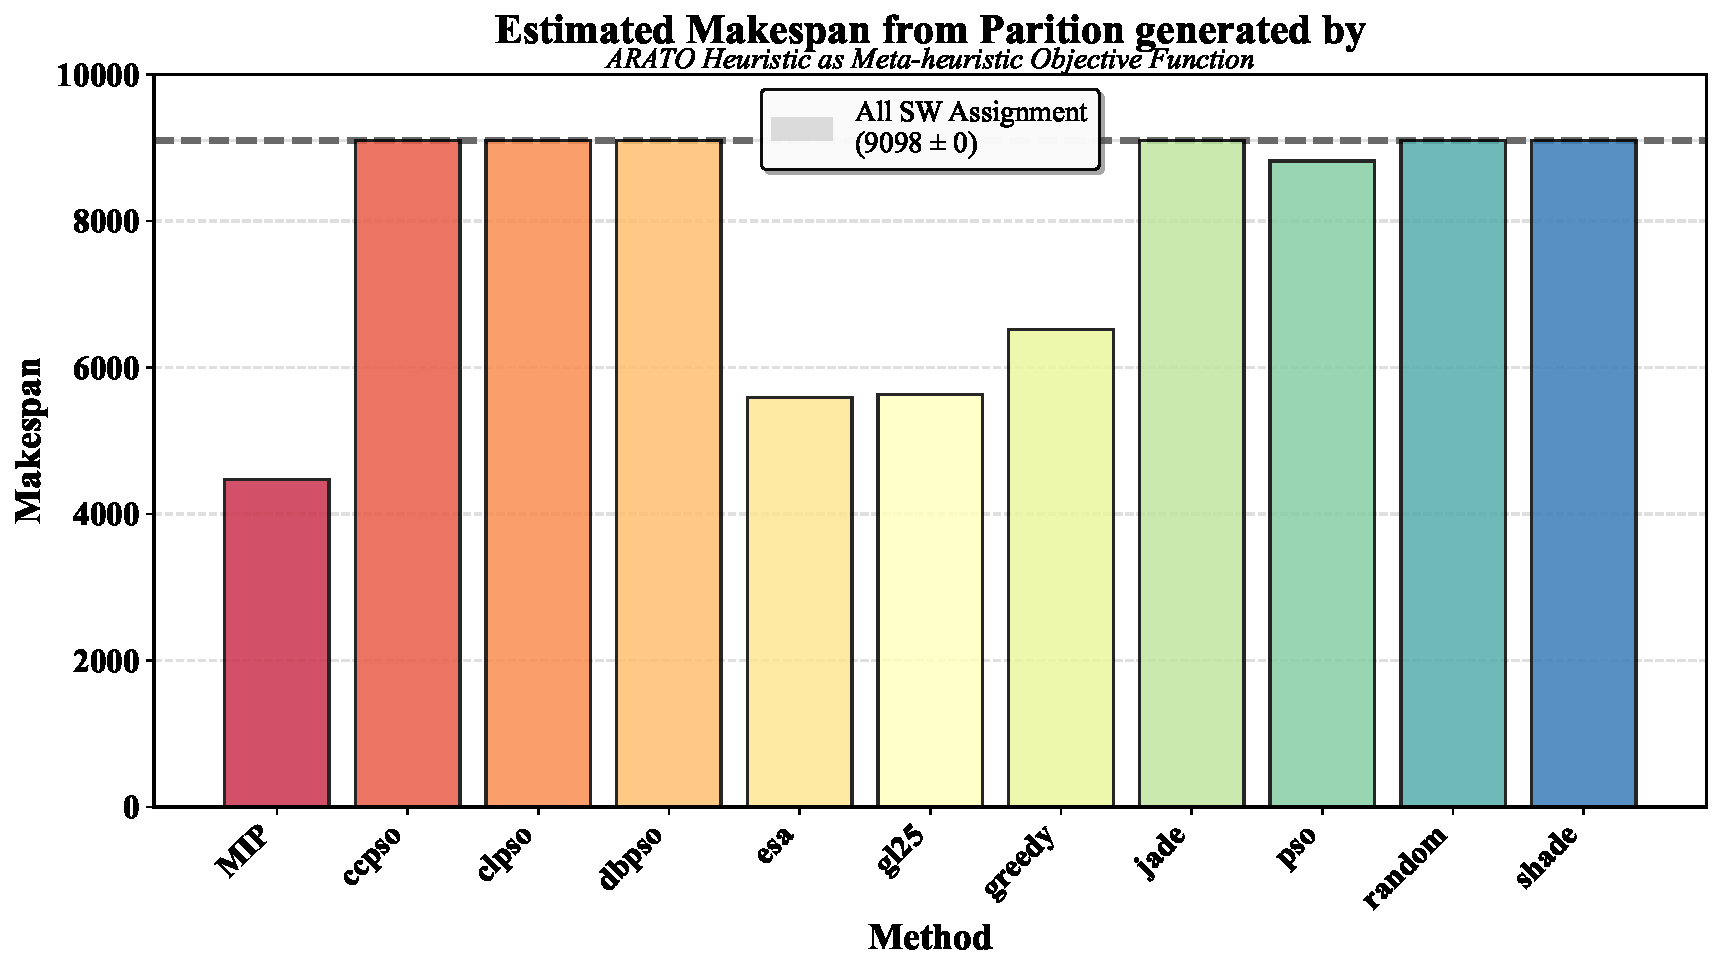
\includegraphics[width=0.48\linewidth]{Figures/meta-heuristic-Figures/arato-results-hw-0.1-area-0.5-seeds0-3-1.pdf}
    }
    \hfill
\subfloat[OPTM Heuristic\label{fig:optm_results}]{
        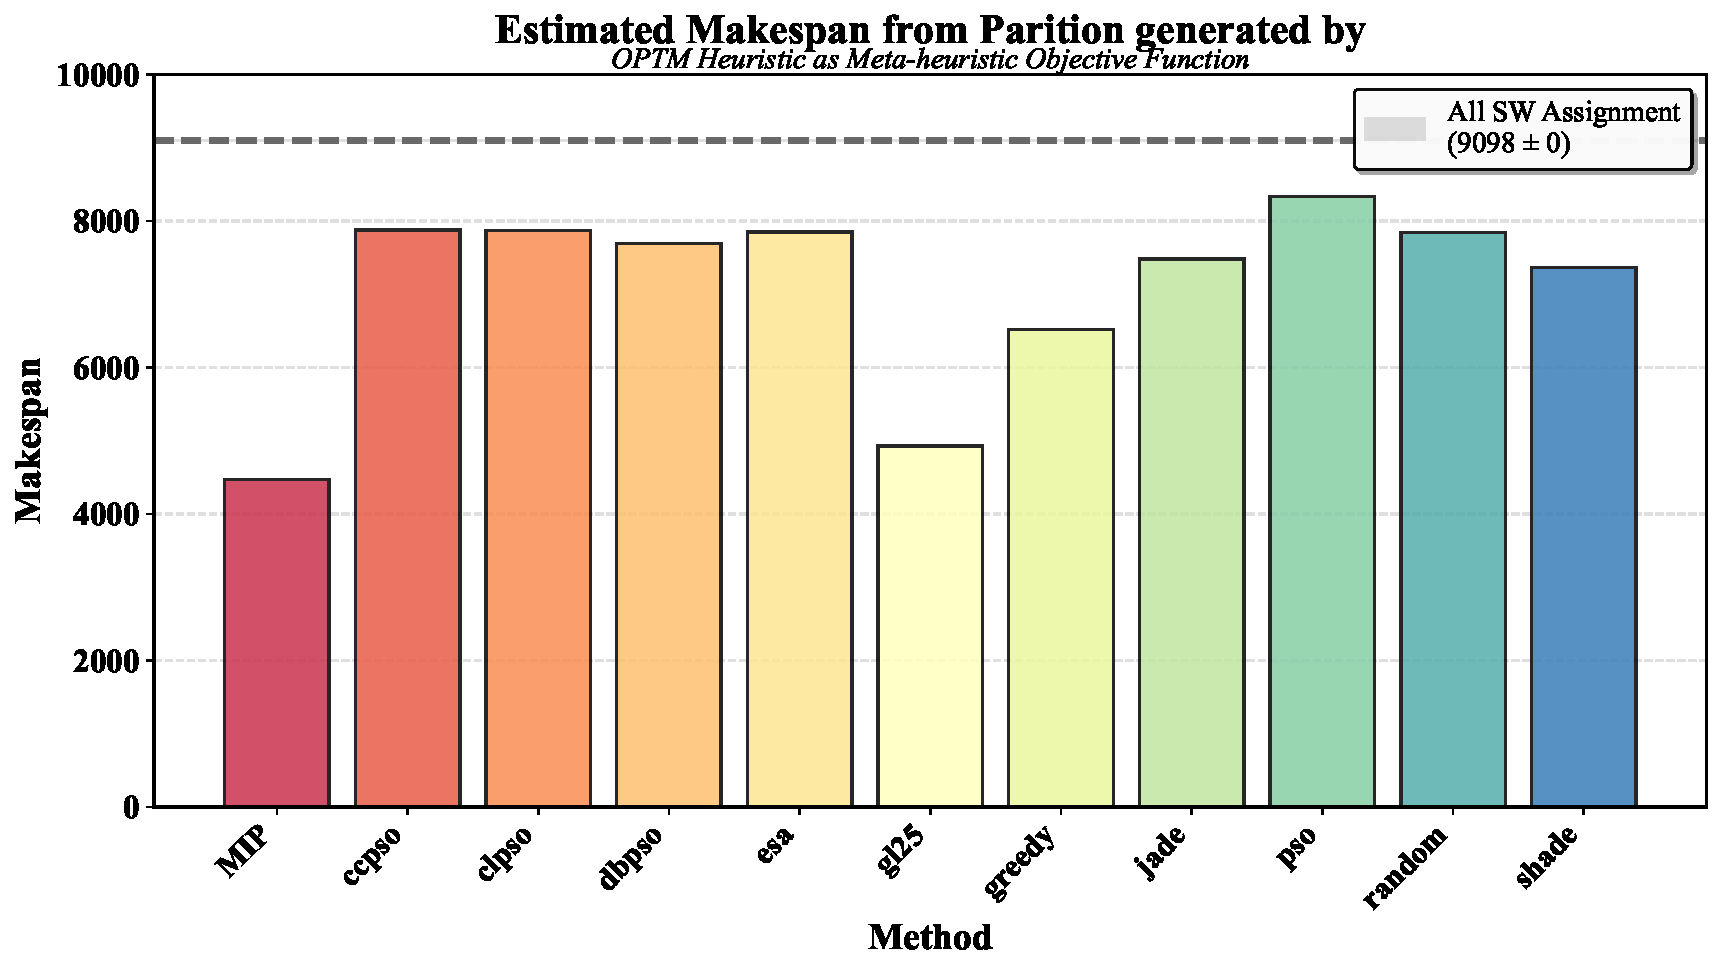
\includegraphics[width=0.48\linewidth]{Figures/meta-heuristic-Figures/makespan-results-hw-0.1-area-0.5-seeds0-3.pdf}
    }
    \hfill
    \subfloat[CA heuristic\label{fig:ca_results}]{
        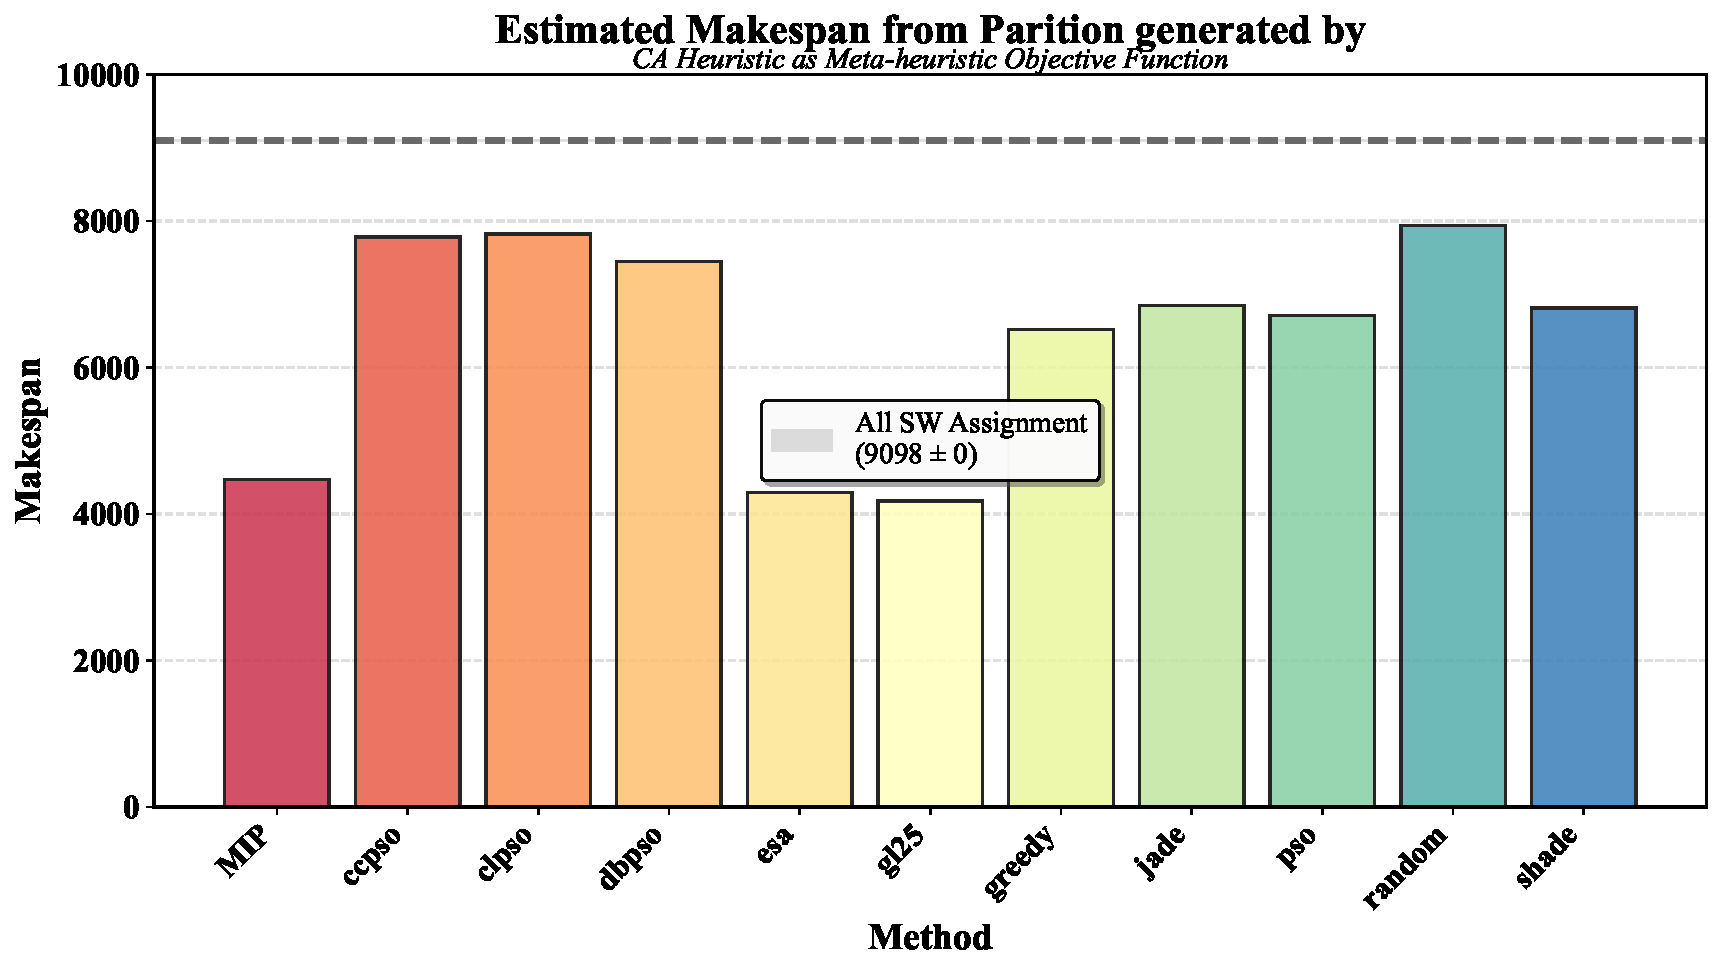
\includegraphics[width=0.48\linewidth]{Figures/meta-heuristic-Figures/comm-results-hw-0.1-area-0.5-seeds0-3.pdf}
    }
    \hfill
        \subfloat[CPL heuristic\label{fig:cpl_results}]{
        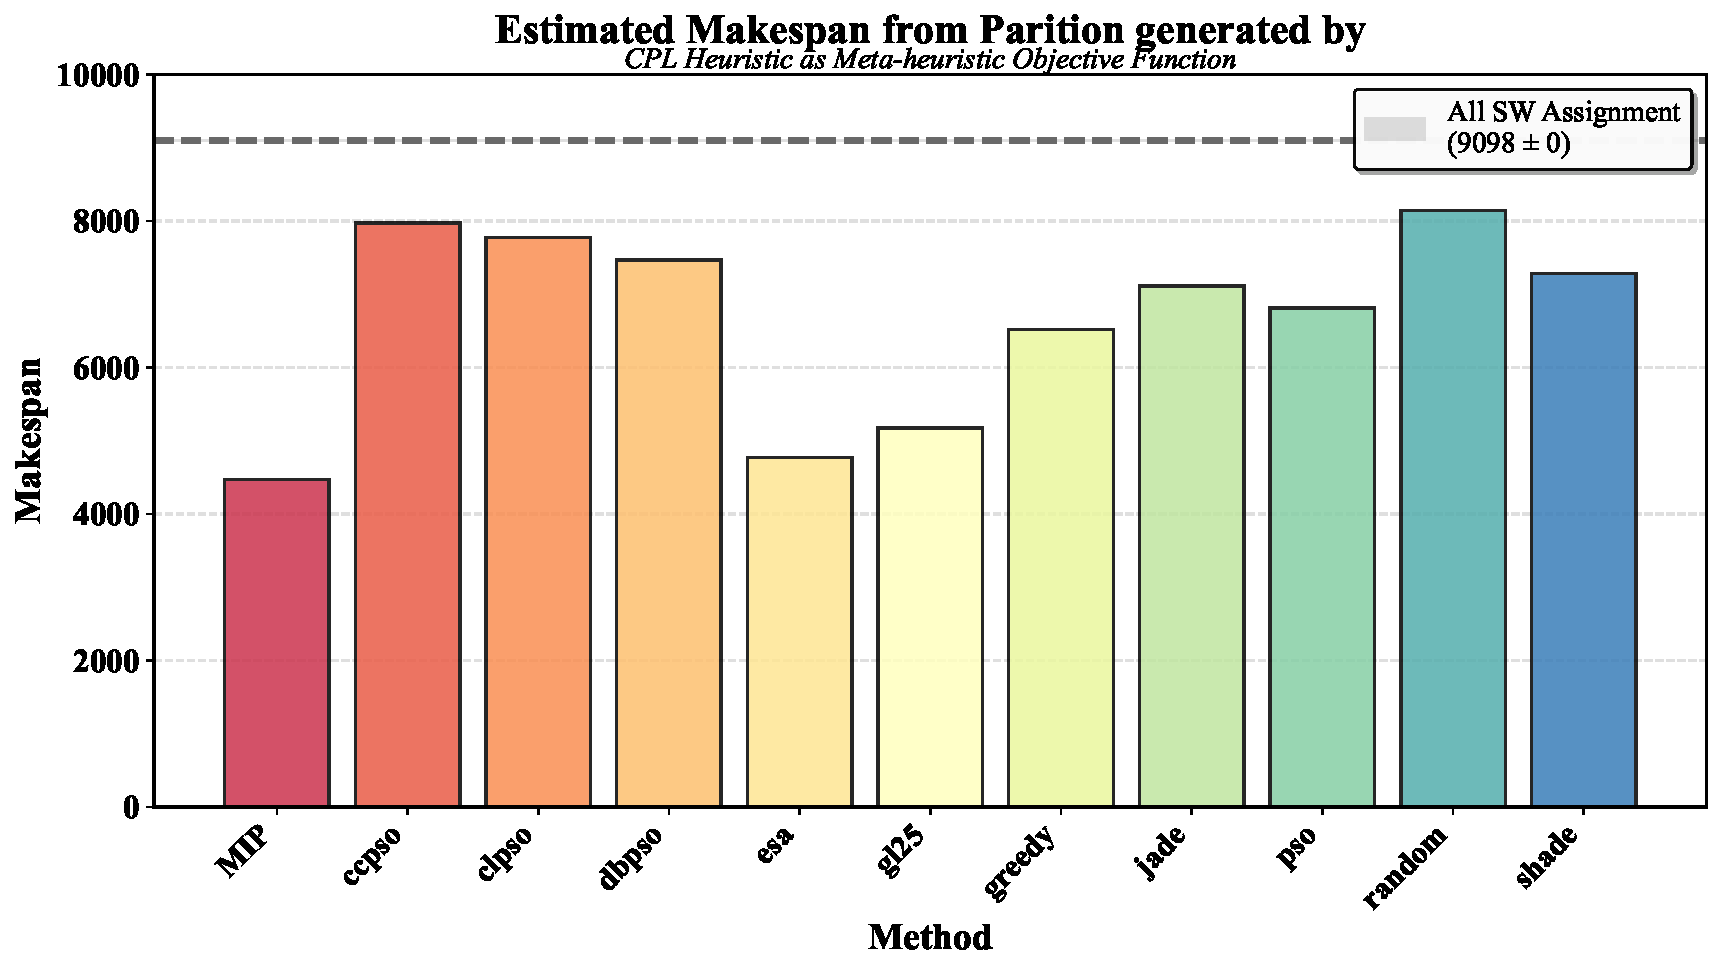
\includegraphics[width=0.48\linewidth]{Figures/meta-heuristic-Figures/cpl-results-hw-0.1-area-0.5-seeds0-3.pdf}
    }
    \hfill
        \subfloat[ED heuristic\label{fig:ed_results}]{
        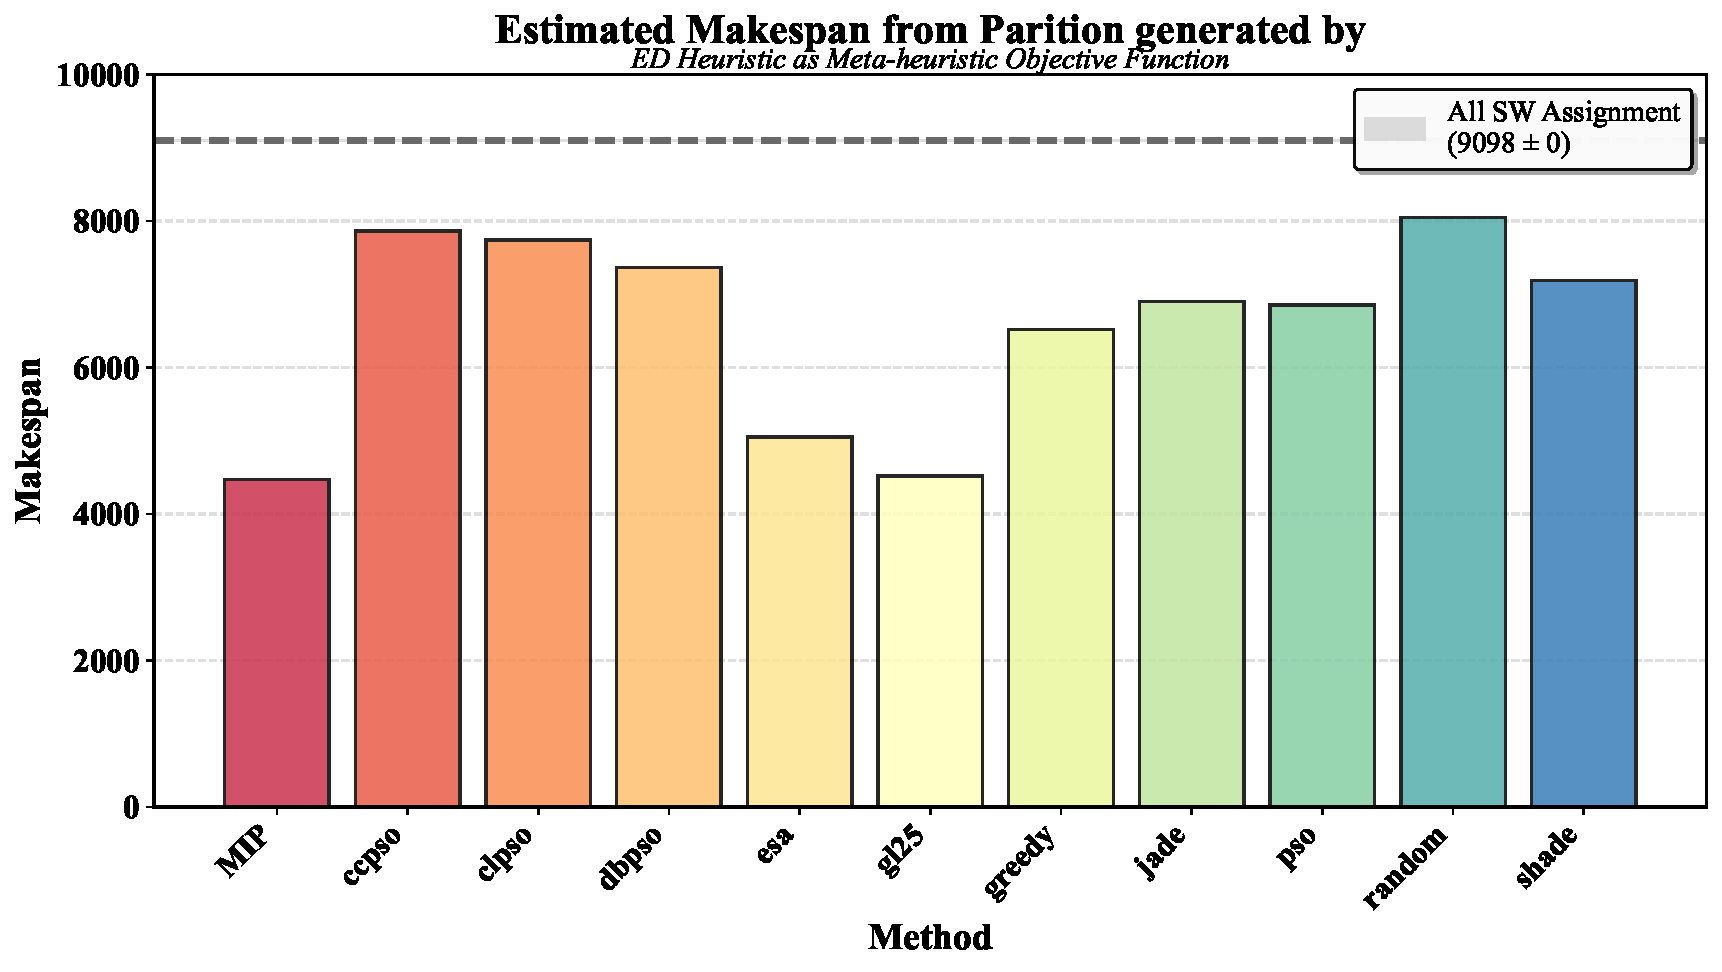
\includegraphics[width=0.48\linewidth]{Figures/meta-heuristic-Figures/ed-results-hw-0.1-area-0.5-seeds0-3.pdf}
    }
    \hfill
        \subfloat[SPT heuristic cost\label{fig:spt_results}]{
        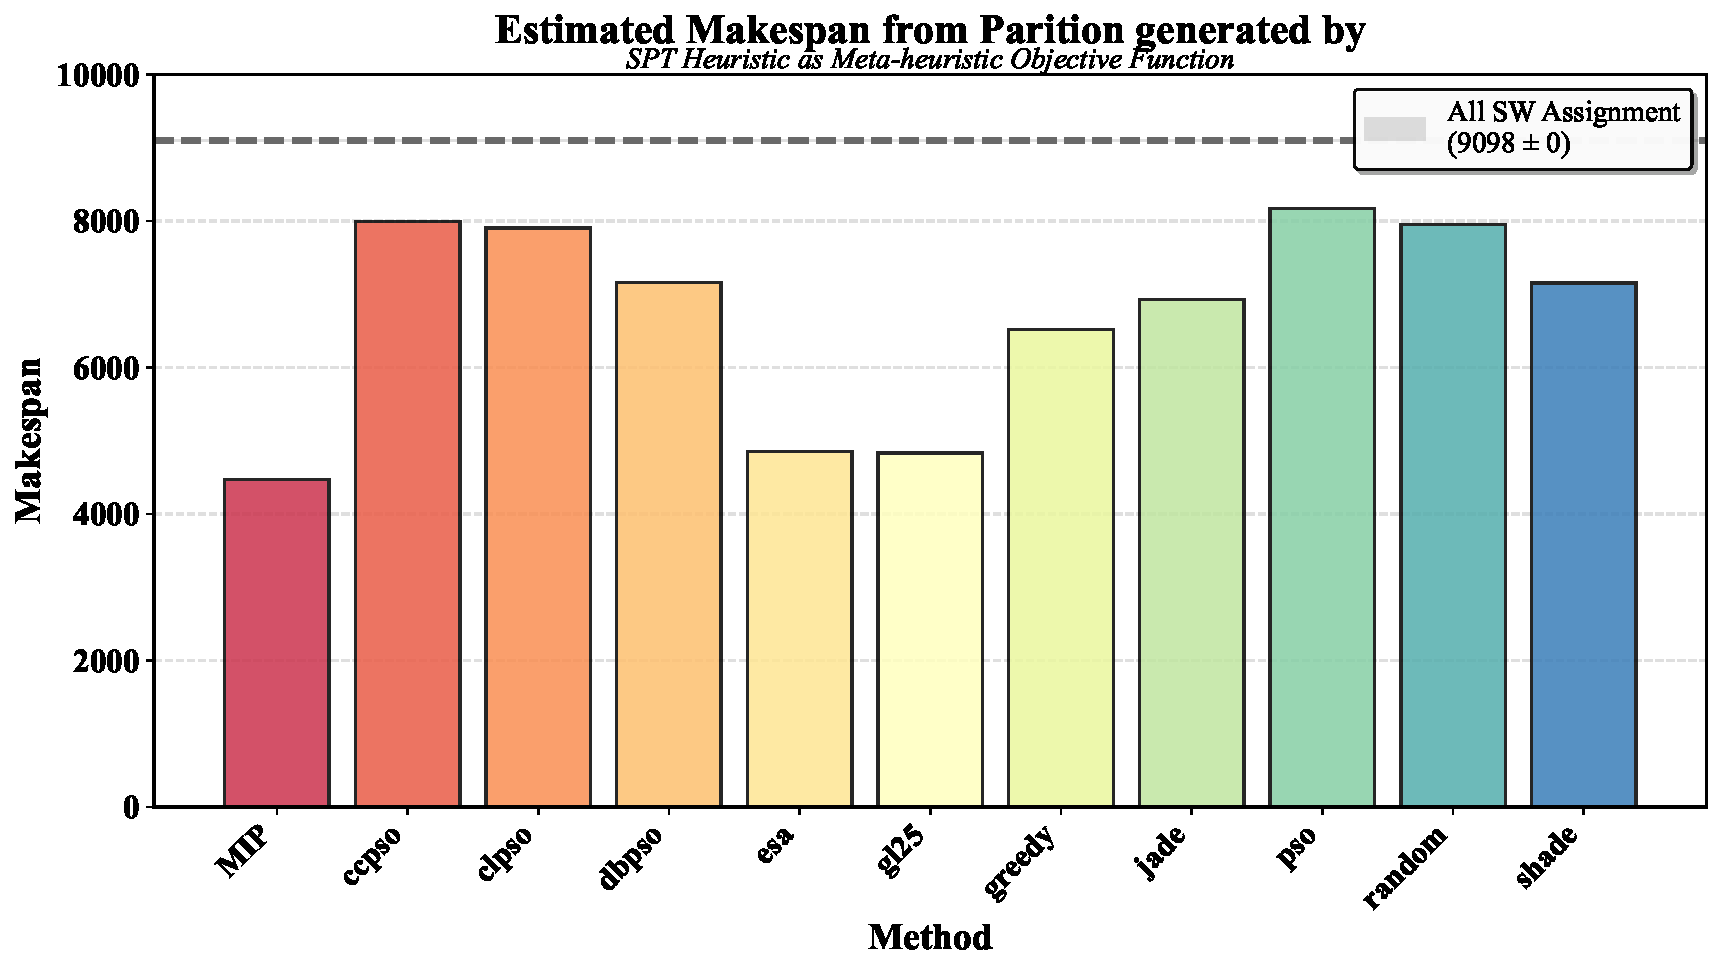
\includegraphics[width=0.48\linewidth]{Figures/meta-heuristic-Figures/spt-results-hw-0.1-area-0.5-seeds0-3.pdf}
    }
    \hfill

    \caption{{Comparison of Various Baseline MetaHeuristics on different optimization functions}}
    \label{fig:metaheur-compare}
    
\end{figure}

\begin{table}
\caption{\% Improvment of MIP over various meta heuristic methods for $k = 0.1, \alpha = 0.5$}
\begin{tabular}{llrrrrrrrr}
\toprule
 opt\_strategy & ccpso & clpso & dbpso & esa & gl25 & jade & pso & shade \\
\midrule
ARATO & 50.87 & 50.87 & 50.87 & 20.0 & 20.63 & 50.87 & 49.31 & 50.87 \\

CA & 42.55 & 42.83 & 40 & -4.16 & -7.05 & 34.68 & 33.38 & 34.37 \\

CPL & 43.94 & 42.5 & 40.14 & 6.35 & 13.55 & 37.18 & 34.39 & 38.6 \\

ED & 43.15 & 42.24 & 39.29 & 11.5 & 1.13 & 35.25 & 34.75 & 37.78 \\

OPTM & 43.27 & 43.21 & 41.91 & 43.05 & 9.35 & 40.27 & 46.38 & 39.29 \\

SPT & 44.09 & 43.44 & 37.56 & 7.94 & 7.56 & 35.45 & 45.30 & 37.45 \\
\bottomrule
\end{tabular}
\label{tab:mip_improvement}
\end{table}


\subsection{Results}

\subsubsection{SqueezeNet, $k=0.1, \alpha=0.5$}

Figure~\ref{fig:metaheur-compare} shows the performance of various methods with respect to various optimization strategies (Random and greedy does not have any).
Table~\ref{tab:mip_improvement} presents the percentage improvement of the Mixed Integer Programming (MIP) solution over various meta-heuristic methods for hardware scale factor $k = 0.1$ and area constraint $\alpha = 0.5$. The results reveal significant variations in performance across different optimization strategies and meta-heuristic algorithms.

\noindent
\textbf{Drawback of ARATO strategy}
The ARATO optimization strategy exhibits the poorest performance for the meta heuristics, with MIP outperforming most meta-heuristics by approximately 50\%, except for ESA (20.0\%) and GL25 (20.63\%). This substantial gap suggests that ARATO-based meta-heuristics struggle to find near-optimal solutions for the given problem constraints.

\noindent
\textbf{Best Performing Meta-Heuristics:}
Across all the optimization strategies, GL25 and ESA consistently demonstrate the smallest performance gaps relative to MIP. Notably, for the CA (Communication-Aware) strategy, both methods achieve superior evaluation metrics compared to MIP. \zmcomment{This is due to MIP jointly solving partitioning and scheduling, and the evaluation function takes a specific scheduling. Thus, the superiority of the MIP may be overlooked here}. This suggests that for communication-intensive objectives, meta-heuristics can explore solution spaces more effectively than exact methods within practical time constraints. --\zmcomment{May not be necessarily true, but given the current nature of evaluation, this is the best I can put}

\noindent
\textbf{Strategy-Specific Observations:}
\begin{itemize}
    \item \textbf{ARATO:} Shows poor performance across PSO variants (PSO, DBPSO, CCPSO, CLPSO, JADE, SHADE), suggesting these methods converge to similar suboptimal regions for this strategy.
    
    \item \textbf{CA (Communication-Aware):} Exhibits the most varied performance, with GL25 and ESA achieving superior solutions to MIP while PSO variants lag by 33--43\%. This indicates that genetic algorithms and simulated annealing better capture the communication cost structure.
    
    \item \textbf{OPTM (Makespan Optimization):} PSO has the largest improvement gap (46.38\%), while GL25 shows exceptional performance with only 9.35\% gap, demonstrating the effectiveness of genetic approaches for scheduling-oriented objectives.
    
    \item \textbf{CPL, ED, and SPT:} These strategies show similar margins, with GL25 and ESA consistently performing better than PSO-based approaches.
\end{itemize}

\textbf{Algorithm Family Comparison:}
\begin{itemize}
    \item \textit{PSO Variants} (PSO, DBPSO, CCPSO, CLPSO): Demonstrate relatively consistent performance within each strategy, with optimality gaps ranging from 33--50\%. CCPSO and CLPSO variations show minimal differentiation from standard PSO.
    
    \item \textit{Differential Evolution} (JADE, SHADE): Perform comparably to PSO variants, with JADE generally achieving slightly better results than SHADE across most strategies.
    
    \item \textit{Genetic Algorithm} (GL25): Stands out as the most competitive meta-heuristic, achieving the smallest gaps across five of six strategies.
    
    \item \textit{Simulated Annealing} (ESA): Shows strong performance particularly in CA and CPL strategies.
\end{itemize}

% Figure~\ref{fig:makespan_results} and Figure~\ref{fig:partition_cost_results} present the comparative performance of all implemented meta-heuristic methods across both objective functions. The results reveal significant performance variations among different algorithmic approaches, with clear distinctions between the effectiveness of various optimization paradigms.

% For makespan minimization, GL25 emerges as the most effective method, achieving an estimated makespan of approximately 4,700 time units, representing a substantial improvement over the all-software baseline of 8,500 units. This corresponds to a makespan reduction of approximately 45\%, demonstrating the significant potential of hardware-software co-design optimization. CLPSO and SHADE also demonstrate competitive performance, achieving makespans around 7,800 time units, while other methods including DBPSO, Random, PSO, JADE, CCPSO, and Greedy cluster around 8,000 time units, showing marginal improvements over the naive all-software assignment. Notably, ESA achieves a makespan of approximately 7,500 units, positioning it in the middle tier of performance.

% In terms of partition cost optimization, the results show a different performance ranking. GL25 again demonstrates superior performance with the lowest partition cost of approximately 7,400 units, significantly outperforming all other methods. CLPSO, SHADE, and ESA achieve competitive results with partition costs ranging from 7,400 to 8,600 units, all maintaining costs below the all-software baseline. Interestingly, the Greedy heuristic produces the highest partition cost at approximately 12,500 units, suggesting that the simple gain-per-area ratio approach may not be optimal for this particular problem configuration. The remaining methods (DBPSO, Random, PSO, JADE, CCPSO) exhibit similar performance levels, clustering around 8,400-8,700 units.

Our first analysis reveals that GL25 and ESA consistently achieve superior performance across all objective functions, establishing it as the most robust methods for this particular task graph configuration.
\zmcomment{Note that ESA,GL25 have higher iterations than many other (except SHADE, JADE)}

\zmcomment{Before proceeding more, we need to decide the following.

\begin{enumerate}
    \item All experimental configurations -- number of environment parameters to evaluate against, how many run per each config.

    \item task graphs -- how many taskgraphs to evaluate against

    \item evaluation functions -- what function to use for evaluation

\end{enumerate}
}



